\documentclass[11pt,a4paper]{article}

\usepackage[utf8]{inputenc}
\usepackage[T1]{fontenc}
\usepackage[margin=2.5cm]{geometry}
\usepackage{amsmath,amssymb}
\usepackage{graphicx}
\usepackage{booktabs}
\usepackage{siunitx}
\usepackage{xcolor}
\usepackage{caption}
\usepackage{subcaption}
\usepackage[numbers,sort&compress]{natbib}
\usepackage{hyperref}

\graphicspath{{figures/}}
\sisetup{group-separator={\,}, group-minimum-digits=4}

% Draft helpers: red notes that are easy to search for and remove later
\newcommand{\todo}[1]{\textcolor{red}{[TODO: #1]}}
\newcommand{\note}[1]{\textcolor{blue}{[NOTE: #1]}}

% Notation
\newcommand{\nD}{n_D}
\newcommand{\nT}{n_T}
\newcommand{\nref}{n_\mathrm{ref}}
\newcommand{\rid}{r_\mathrm{ideal}}
\newcommand{\rhat}{\hat r}
\newcommand{\lavg}{\lambda_\mathrm{avg}}

\title{Extremum Seeking Control for D--T Fuel Ratio Optimisation:\\
       Parameter Study on a First-Order Density Model\\[0.5ex]
       \large Working report (draft)}
\author{Phuc \todo{full name} \\ Supervisor: Juan Javier Palacios Roman}
\date{\today}

\begin{document}
\maketitle

\begin{abstract}
Fusion power in a D--T plasma scales with the product $\nD\nT$. At fixed total density, this product is maximal when the two species have equal density. The fuel ratio that achieves this, $\rid=\alpha_T/(\alpha_T+\alpha_D)$, depends on the particle loss rates. These rates are not known accurately and may drift in time.
We study a sinusoidal-perturbation extremum seeking controller (ESC) that tunes the tritium fraction $r$ of the gas puff online. The plant is a two-species first-order density model with a PI controller on the total density.
Large random parameter sweeps (up to $2\times10^5$ simulations per sweep) over optimizer gain $k$, dither amplitude $a$ and dither frequency $f$ show three things. First, the convergence time is organised mainly by a single combined rate, $\lavg = 2\nref^2\,k\,c(\omega)$, which follows from averaging theory. In the window $0.1\lesssim\lavg\lesssim\SI{3}{s^{-1}}$, \SI{96}{\percent} of runs converge. Second, the energy lost to the dither is predicted well by a closed-form estimate. This loss is negligible at high dither frequency because the plasma density responds as a low-pass filter. Third, compared with keeping $r=0.5$ fixed, a well-tuned ESC delivers more energy in \SIrange{93}{99}{\percent} of cases. However, the attainable gain is bounded by $(1-2\rid)^2$ of the output for a static plant, which is at most \SI{1}{\percent} in the range studied. Up to \SI{5}{\percent} is attainable when $\rid$ drifts. In this simple model, ESC is therefore worth using mainly when $\rid$ is uncertain or time-varying, and only if it is tuned inside the window identified here.
\end{abstract}

\tableofcontents

%======================================================================
\section{Introduction}
%======================================================================

The fusion power density of a D--T plasma is
\begin{equation}
  P_\mathrm{fus} \propto \nD\,\nT\,\langle\sigma v\rangle(T),
\end{equation}
so at fixed temperature the power is set by the product of the deuterium and tritium densities \citep{wesson2004tokamaks}.
The total density cannot be raised indefinitely: it is bounded by the Greenwald limit $n_\mathrm{GW}$ \citep{greenwald2002density}, and in practice a reference $\nref<n_\mathrm{GW}$ is chosen and held by a density controller.
With $\nD+\nT=\nref$ fixed, $\nD\nT=\nT(\nref-\nT)$ is maximal at $\nD=\nT=\nref/2$, where $\nD\nT=\nref^2/4$.

The actuator is the fuelling: a total puff rate $S$ split into tritium and deuterium with \emph{fuel ratio}
\begin{equation}
  r = \frac{\Gamma_T}{\Gamma_T+\Gamma_D}\in[0,1].
\end{equation}
Because D and T are lost at different rates, the ratio that equalises the densities is generally not $0.5$, and the loss rates are neither known precisely nor constant.
Extremum seeking control (ESC) \citep{krstic2000stability,ariyur2003realtime,tan2010extremum} is a model-free, online optimiser: it perturbs $r$, measures the response of a signal proportional to $\nD\nT$ (in practice the neutron rate), and climbs the estimated gradient.

This report records the findings of the first project phase, which uses a deliberately simple plant. The questions are:
\begin{enumerate}
  \item How do the ESC parameters (optimizer gain $k$, dither amplitude $a$, dither frequency $f$) affect \emph{whether} and \emph{how fast} the controller converges to $\rid$? (``Safe-to-operate'', STO.)
  \item How do they affect the \emph{energy} produced, and when is ESC better than simply operating at $r=0.5$? (``Optimal-to-operate'', OTO.)
  \item Can a small neural-network classifier predict these outcomes from the ESC parameters?
\end{enumerate}
More complex plants (nonlinear dynamics, noise, delays, discrete-time ESC, alternative optimisers such as RMSprop \citep{tieleman2012rmsprop}) are planned for later phases (Section~\ref{sec:outlook}).

%======================================================================
\section{Plant model}
\label{sec:model}
%======================================================================

\subsection{Two-species density dynamics}
Following the initial material supplied by the supervisor (\texttt{main\_fuelratio.m}, \texttt{sim\_fuelratio.slx}), each species obeys a first-order particle balance,
\begin{align}
  \dot n_D &= -\alpha_D\, n_D + \Gamma_D, & \Gamma_D &= (1-r)\,S,\\
  \dot n_T &= -\alpha_T\, n_T + \Gamma_T, & \Gamma_T &= r\,S,
\end{align}
with loss rates $\alpha_D=1/\SI{1.71}{s}$ and $\alpha_T=1/\SI{1.66}{s}$ (particle confinement times \SI{1.71}{s} and \SI{1.66}{s}).
Densities are in units of \SI{e19}{m^{-3}} (the factor $10^{19}$ is dropped in the code).
The total puff rate is set by a PI controller on the total density,
\begin{equation}
  S = \max\!\Big(0,\; K_p\,e + K_i\!\int_0^t e\,\mathrm{d}t'\Big),\qquad e=\nref-(\nD+\nT),
\end{equation}
with $K_p=3.129$, $K_i=2.482$, $\nref=11.5$ and $n_\mathrm{GW}=11.9$.
The system is discretised with a zero-order hold at $\Delta t=\SI{0.01}{s}$ and simulated for $t_\mathrm{end}=\SI{100}{s}$.
All runs start from $\nD(0)=0.25(1-0.1)\nref$, $\nT(0)=0.25\cdot0.1\,\nref$, i.e.\ at \SI{25}{\percent} of the reference density.

\subsection{Ideal fuel ratio and the static map}
In steady state $\nT=rS/\alpha_T$ and $\nD=(1-r)S/\alpha_D$. Equal densities require
\begin{equation}
  \rid = \frac{\alpha_T}{\alpha_T+\alpha_D}, \label{eq:rideal}
\end{equation}
which for the nominal rates gives $\rid = 1.71/(1.71+1.66)\approx 0.507$.
With the total held at $\nref$, the steady-state product as a function of $r$ is
\begin{equation}
  J(r)\equiv \nD\nT = \nref^2\,x(1-x),\qquad x=\frac{r/\alpha_T}{r/\alpha_T+(1-r)/\alpha_D},
  \label{eq:staticmap}
\end{equation}
a concave map with maximum $J^\ast=\nref^2/4\approx 33.06$ at $r=\rid$. For $\alpha_D=\alpha_T$ it reduces to $J=\nref^2 r(1-r)$, the parabola in Fig.~\ref{fig:gradient}.

\subsection{Time-varying ideal ratio (OTO studies)}
To mimic slowly changing wall conditions, the OTO scripts prescribe
\begin{equation}
  \rid(t) = r_{\mathrm{ideal},0}\,e^{\lambda t},\qquad
  \alpha_T(t) = \rid(t)\,A,\quad \alpha_D(t)=\big(1-\rid(t)\big)A,\quad A=\tfrac{1}{1.71}+\tfrac{1}{1.66},
  \label{eq:drift}
\end{equation}
so the sum of loss rates is constant and Eq.~\eqref{eq:rideal} holds at every instant.
The sweeps draw $r_{\mathrm{ideal},0}\in[0.45,0.55]$ and $\lambda\in[-0.002,0.002]\,\si{s^{-1}}$. At the extremes, the ratio drifts to $0.55\,e^{0.2}\approx0.67$ or $0.45\,e^{-0.2}\approx0.37$ by $t=\SI{100}{s}$. Over a run, the drift is therefore larger than the spread of initial values.

\paragraph{Cost of a fixed ratio.} Inserting $r=0.5$ into Eq.~\eqref{eq:staticmap} with the parametrisation~\eqref{eq:drift} gives $x=1-\rid$, hence
\begin{equation}
  \frac{J^\ast - J(0.5)}{J^\ast} = (1-2\rid)^2 .
  \label{eq:fixedloss}
\end{equation}
For $\rid=0.475$ or $0.525$ this is \SI{0.25}{\percent}; for $0.45$ or $0.55$ it is \SI{1}{\percent}. \textbf{This is the entire margin ESC can win in a static plant}; it sets the scale for every energy comparison below.

%======================================================================
\section{Extremum seeking controller}
\label{sec:esc}
%======================================================================

\subsection{Loop structure}
The loop is shown in Fig.~\ref{fig:escdiagram}. The applied ratio is
$r(t)=\rhat(t)+a\sin\omega t$ (clipped to $[0,1]$), $\omega=2\pi f$.
The measured product $J=\nD\nT$ passes a high-pass filter $s/(s+\omega_h)$ that removes its mean, is demodulated by $(2/a)\sin\omega t$, and is low-pass filtered by $\omega_l/(s+\omega_l)$ to give the gradient estimate $\xi\approx \mathrm{d}J/\mathrm{d}r$. The integrator $k/s$ updates the estimate, $\dot{\rhat}=k\,\xi$ (also clipped to $[0,1]$).
In all scripts the filter cut-offs are tied to the dither, $\omega_h=\omega_l=\omega/\pi$, so the free ESC parameters are $(k,a,f)$ plus the initial estimate $\rhat_0$.

\begin{figure}[t]
  \centering
  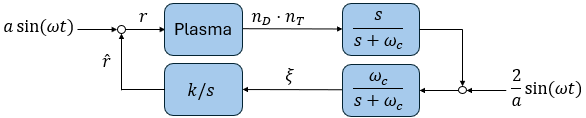
\includegraphics[width=0.85\linewidth]{esc_diagram.png}
  \caption{Sinusoidal-perturbation ESC loop used in this work. The plasma block contains the two-species density model and the PI total-density controller of Section~\ref{sec:model}.}
  \label{fig:escdiagram}
\end{figure}

\begin{figure}[t]
  \centering
  \begin{subfigure}{0.48\linewidth}
    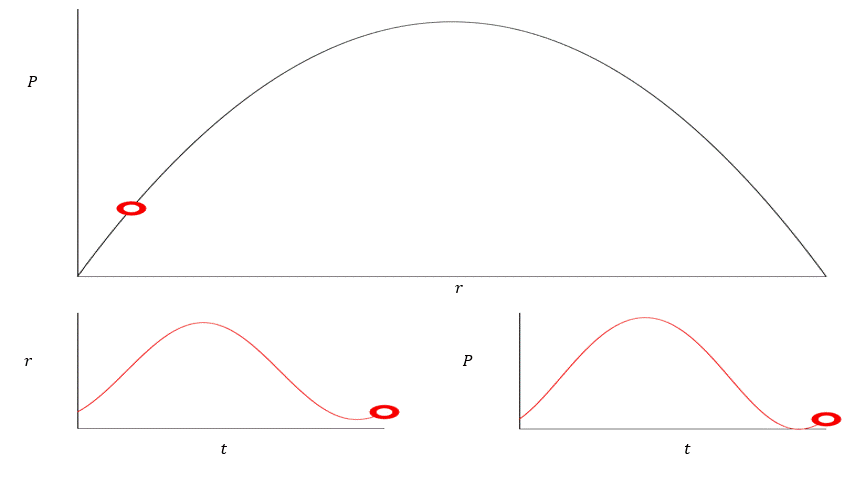
\includegraphics[width=\linewidth]{gradient_in_phase.png}
    \caption{Left of the optimum: $r$ and $P$ in phase ($\mathrm{d}P/\mathrm{d}r>0$).}
  \end{subfigure}\hfill
  \begin{subfigure}{0.48\linewidth}
    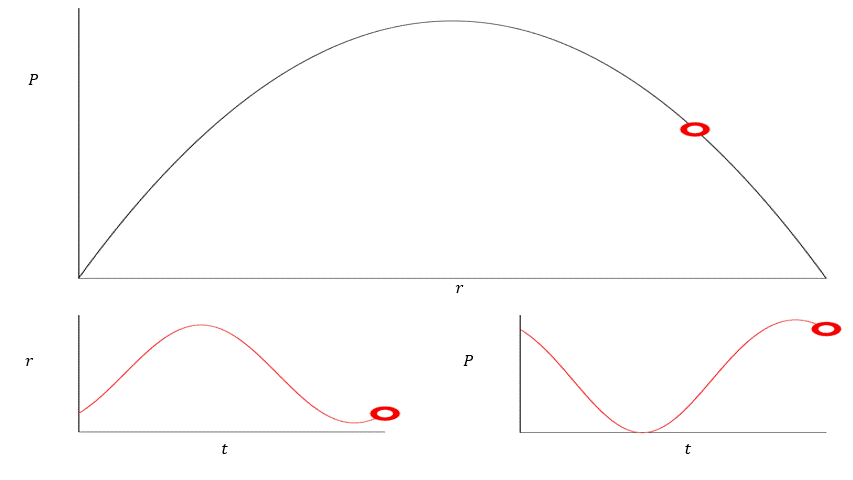
\includegraphics[width=\linewidth]{gradient_anti_phase.png}
    \caption{Right of the optimum: $r$ and $P$ in anti-phase ($\mathrm{d}P/\mathrm{d}r<0$).}
  \end{subfigure}
  \caption{Intuition behind gradient estimation by dithering: the phase between the perturbation $r(t)$ and the response $P(t)$ gives the sign of the local gradient. (Final frames of the animations in \texttt{Theory/Figures}.)}
  \label{fig:gradient}
\end{figure}

\subsection{Averaged dynamics: an effective convergence rate}
\label{sec:averaging}
\note{This subsection is an analysis added while drafting; it explains the sweep results in Section~\ref{sec:sto}. It should be checked by the supervisor.}

For near-equal loss rates, write $\Sigma=\nD+\nT$ and $\Delta=\nT-\nD$. Then $J=(\Sigma^2-\Delta^2)/4$. With $\Sigma$ held at $\nref$ by the PI loop, and $S\approx\bar\alpha\nref$ with $\bar\alpha=(\alpha_D+\alpha_T)/2\approx\SI{0.594}{s^{-1}}$,
\begin{equation}
  \dot\Delta = -\bar\alpha\,\Delta + (2r-1)\,S ,
\end{equation}
so the split responds to $r$ through a first-order low-pass with corner $\bar\alpha$. Linearising $J$ around $\rhat$, the dither component of $J$ reaching the demodulator is the static gradient $J'(\rhat)=\nref^2(1-2\rhat)$ multiplied by $G(j\omega)H(j\omega)$. Here $G(s)=\bar\alpha/(s+\bar\alpha)$ is the normalised plant response and $H(s)=s/(s+\omega_h)$ is the high-pass filter. After demodulation and low-pass filtering,
\begin{equation}
  \xi \approx c(\omega)\,J'(\rhat),\qquad
  c(\omega)=|G(j\omega)H(j\omega)|\cos\varphi,\quad
  \varphi = -\arctan\frac{\omega}{\bar\alpha}+\arctan\frac{\omega_h}{\omega}.
  \label{eq:c}
\end{equation}
With $\omega_h=\omega/\pi$, $|H|=(1+\pi^{-2})^{-1/2}$ and $\arctan(\omega_h/\omega)=\arctan(1/\pi)$. The averaged estimator dynamics are then linear,
\begin{equation}
  \dot{\rhat} \approx -\lavg\,(\rhat-\rid),\qquad \boxed{\lavg = 2\,\nref^2\,k\,c(\omega)} ,
  \label{eq:lavg}
\end{equation}
and the time to enter a \SI{5}{\percent} band starting from $\rhat_0=0$ is $t_\mathrm{conv}\approx\ln 20/\lavg$.
Two consequences:
\begin{itemize}
  \item \textbf{The dither amplitude drops out} to first order, because the demodulation gain $2/a$ cancels the response amplitude $\propto a$.
  \item \textbf{Gain and frequency are coupled}. Above the plant corner, $c(\omega)$ falls steeply: $c=0.57$ at \SI{0.1}{Hz}, $0.084$ at \SI{0.5}{Hz}, and $4.8\times10^{-3}$ at \SI{6}{Hz}. A higher dither frequency therefore needs a proportionally larger $k$. This is the positive $k$--$f$ correlation visible in the sweep pair plots (Fig.~\ref{fig:pairplot}).
\end{itemize}
As a check, the supervisor's default parameters ($k=3\times10^{-4}$, $a=0.1$, $f=\SI{0.1}{Hz}$) give $\lavg=\SI{0.045}{s^{-1}}$ and $t_\mathrm{conv}\approx\SI{66}{s}$. This is consistent with the $\approx\SI{60}{s}$ observed with \texttt{main\_fuelratio.m}. For $k=4\times10^{-4}$ (\texttt{ESC.m}) the estimate is \SI{50}{s} (cf.\ Fig.~\ref{fig:example}).
The averaging argument assumes time-scale separation. It must fail when $\lavg$ approaches the low-pass cut-off $\omega_l$ or the plant rate, and it ignores the start-up transient of the PI loop.

\subsection{Steady-state cost of the dither}
\label{sec:ditherloss}
Because $J$ is concave, any oscillation of $\Delta$ lowers its mean. With $\Delta$ oscillating at amplitude $2\bar\alpha\nref a/\sqrt{\bar\alpha^2+\omega^2}$, the mean loss in $J$ is
\begin{equation}
  \frac{\delta J}{J^\ast} = \frac{2a^2\bar\alpha^2}{\bar\alpha^2+\omega^2},\qquad
  L_\mathrm{dith} = T\,\frac{\nref^2}{4}\,\frac{2a^2\bar\alpha^2}{\bar\alpha^2+\omega^2}
  \label{eq:ditherloss}
\end{equation}
over a run of length $T$. For the default dither ($a=0.1$, \SI{0.1}{Hz}) the loss is \SI{0.94}{\percent} of the output. This is as large as the whole fixed-ratio margin of Eq.~\eqref{eq:fixedloss}. For $a=0.2$ at \SI{6}{Hz} it is $2\times10^{-5}$ of the output. The plasma low-pass therefore makes high dither frequencies almost free in energy terms; their price is the large gain they need (Eq.~\eqref{eq:lavg}).

%======================================================================
\section{Simulation campaigns and metrics}
\label{sec:setup}
%======================================================================

\paragraph{Convergence.} A run is \emph{converged} if $|\rhat-\rid(t)|\le0.05\,\rid(t)$ continuously for \SI{5}{s}. The convergence time is the start of the first such interval. Non-converged runs have no convergence time (NaN). Because of the hold time, convergence times are censored at \SI{95}{s}.

\paragraph{Energy.} $E=\int_0^{T}\nD\nT\,\mathrm{d}t$ (trapezoidal rule), in code units (densities in \SI{e19}{m^{-3}}, time in s). Since $\langle\sigma v\rangle$ is constant, this is proportional to the fusion energy. Each OTO run also simulates the same plant with $r\equiv0.5$ and no ESC, giving $E_{r=0.5}$. The label \texttt{choose\_ESC} is $1$ if $E_\mathrm{ESC}>E_{r=0.5}$.
The scripts also store $E_\mathrm{max}=T\nref^2/4=3306.25$. This value is \emph{not attainable}, because every run starts at \SI{25}{\percent} density. The largest ESC energy in any sweep is $E_\mathrm{ceil}=3293.9$ (\SI{99.63}{\percent} of $E_\mathrm{max}$). We use $E_\mathrm{ceil}-E_{r=0.5}$ as the practical upper bound on the ESC gain.

\paragraph{Parameter sampling.} $k$ is drawn log-uniformly, $a$ and $f$ uniformly. Table~\ref{tab:datasets} lists the data sets used.

\begin{table}[t]
  \centering
  \small
  \caption{Simulation data sets in the repository used in this report. STO: $\rhat_0=0$, constant plant unless stated. OTO: $\rhat_0=0.5$, plant drifting according to Eq.~\eqref{eq:drift}.}
  \label{tab:datasets}
  \begin{tabular}{@{}llrlll@{}}
    \toprule
    Data set (CSV) & Script & Runs & $k$ & $a$ & $f$ [Hz] \\
    \midrule
    \texttt{STO-const\_decay-200k} & \texttt{STO\_ESC\_constdecay.m} & \num{200000} & $[10^{-5},5]$ & $(0,1]$ & $(0,10]$ \\
    \texttt{STO-random\_decay}$^{a}$ & \texttt{STO\_ESC\_randdecay.m} & \num{10000} & $[10^{-5},10^{-2}]$ & $[0.01,0.5]$ & $[0.01,0.5]$ \\
    \texttt{STO-const\_decay-10k}$^{b}$ & (earlier version) & \num{10000} & $[10^{-3},0.1]$ & $[0.01,0.5]$ & $[0.4,0.8]$ \\
    \texttt{OTO-ESC-200k} & \texttt{OTO\_ESC\_rand\_Plant\_rand.m} & \num{200000} & $[10^{-5},5]$ & $(0,1]$ & $(0,10]$ \\
    \texttt{OTO-ESC\_fix-1\_0.2\_6} & \texttt{OTO\_ESC\_fix\_Plant\_rand.m} & \num{100000} & $1$ & $0.2$ & $6$ \\
    \texttt{OTO-Plant\_fix-*} (6 plants) & \texttt{OTO\_ESC\_rand\_Plant\_fix.m} & $6\times\num{100000}$ & $[10^{-5},5]$ & $(0,1]$ & $(0,10]$ \\
    \bottomrule
  \end{tabular}\\[0.5ex]
  \raggedright\footnotesize
  $^{a}$ Loss times randomised by $\pm\SI{0.1}{s}$ per run; D/T actuators swapped in this script (see Section~\ref{sec:issues}).\quad
  $^{b}$ In \texttt{Safe-to-operate/STO-const\_decay/Mistakes}; further exploratory sweeps (100k--550k) are in the same folder.
\end{table}

%======================================================================
\section{Results}
\label{sec:results}
%======================================================================

\subsection{A single ESC run}
Figure~\ref{fig:example} shows a run of \texttt{ESC.m} ($k=4\times10^{-4}$, $a=0.1$, $f=\SI{0.1}{Hz}$, $\rhat_0=0$). The PI loop brings $\nD+\nT$ to $\nref$ within a few seconds, so ESC only has to fix the split. $\rhat$ rises monotonically and enters the \SI{5}{\percent} band after roughly \SI{40}{s}--\SI{45}{s} \todo{read exact value from the run}. $\nD\nT$ climbs to $\approx33$ with a visible ripple caused by the dither. At this low dither frequency the ripple is the dither loss of Eq.~\eqref{eq:ditherloss}.

\begin{figure}[t]
  \centering
  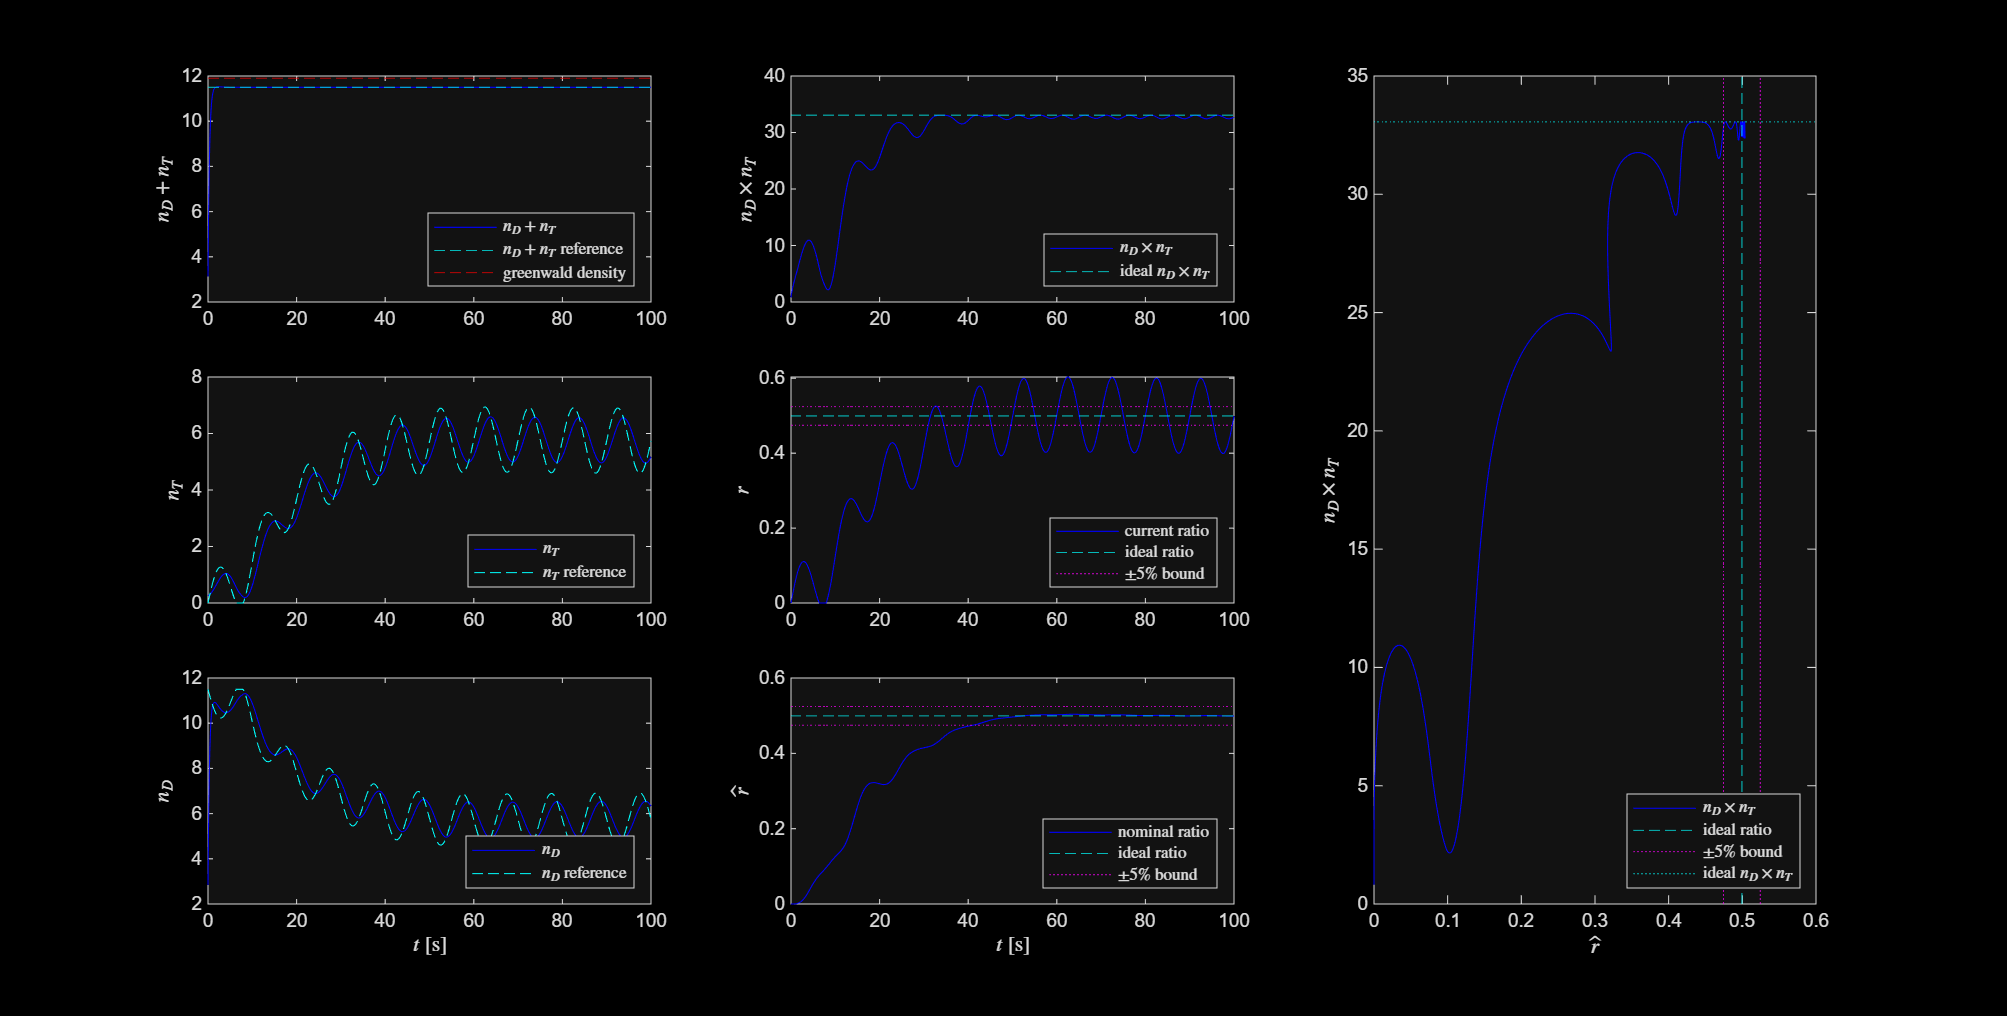
\includegraphics[width=\linewidth]{example_esc_run.png}
  \caption{Example run of \texttt{ESC.m}. Left: total, T and D densities. Middle: $\nD\nT$, applied ratio $r$ and estimate $\rhat$ with the $\pm\SI{5}{\percent}$ band around $\rid$. Right: $\nD\nT$ versus $\rhat$. \todo{re-export with white background for print.}}
  \label{fig:example}
\end{figure}

\subsection{Safe-to-operate: convergence versus ESC parameters}
\label{sec:sto}

\paragraph{Raw parameter dependence.} In the broad 200k sweep, \SI{36.9}{\percent} of runs converge. The median convergence time of converged runs is \SI{14.4}{s}; \num{12465} runs converge within \SI{10}{s} and \num{138} within \SI{5}{s}. The fastest run takes \SI{2.25}{s} ($k=1.42$, $a=0.88$, $f=\SI{1.74}{Hz}$).
Among converged runs, the Spearman rank correlation with convergence time is $-0.45$ for $k$, $-0.21$ for $f$ and $+0.05$ for $a$. The gain dominates, the frequency matters, and the amplitude barely matters.
The earlier 10k sweep shows the same pattern in a narrower box (Fig.~\ref{fig:pairplot}). Among runs that converge in under \SI{10}{s}, fast convergence requires $k$ to increase with $f$, while $a$ is spread over its full range.

\begin{figure}[t]
  \centering
  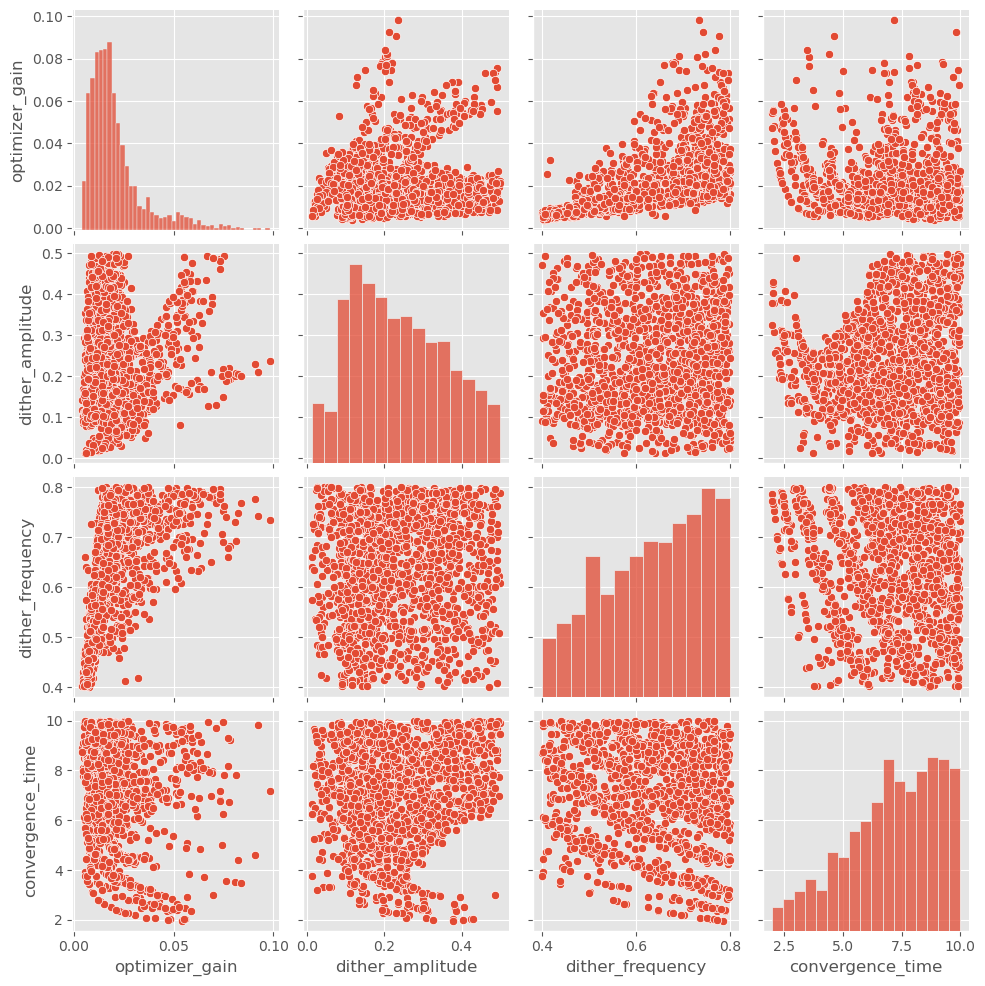
\includegraphics[width=0.7\linewidth]{pairplot_conv_time_lt10.png}
  \caption{Pair plot of runs with convergence time $<\SI{10}{s}$ from the 10k constant-decay sweep ($k\in[10^{-3},0.1]$, $a\in[0.01,0.5]$, $f\in[0.4,0.8]$\,Hz). Note the band structure in $k$ versus $f$: faster dithers require larger gains. Figure from the repository.}
  \label{fig:pairplot}
\end{figure}

\paragraph{Collapse onto the averaged rate.} Re-expressing each run of the 200k sweep through $\lavg$ (Eq.~\eqref{eq:lavg}) organises the data (Fig.~\ref{fig:sto}):
\begin{itemize}
  \item For $\lavg\lesssim\SI{0.01}{s^{-1}}$ no run converges within \SI{100}{s}: the controller is too slow.
  \item In the window $0.1\le\lavg\le\SI{3}{s^{-1}}$ (\SI{25.9}{\percent} of the sweep), \SI{96.3}{\percent} of runs converge, with median times of \SIrange{10.7}{13.3}{s}.
  \item Above $\lavg\approx\SI{10}{s^{-1}}$ only \SI{1.1}{\percent} converge: the loop is too fast for the averaging assumption and oscillates or saturates at the bounds of $r$.
\end{itemize}
At low $\lavg$ the measured times follow the trend of $\ln20/\lavg$, lying somewhat below it because only the faster runs finish within \SI{100}{s}. At high $\lavg$ they saturate at $\approx\SI{10}{s}$, a floor set by the PI start-up transient and the filter lags, which the averaged model neglects. Inside the window, the dither frequency still matters: \SI{99.9}{\percent} converge for $f\in[5,10]$\,Hz but only \SI{23}{\percent} for $f\le\SI{0.05}{Hz}$, because averaging needs $\omega$ to be well separated from the closed-loop rate. The amplitude has a small effect except for $a\lesssim0.05$, where the convergence fraction drops to \SI{82}{\percent} (Fig.~\ref{fig:sto}c).

\begin{figure}[t]
  \centering
  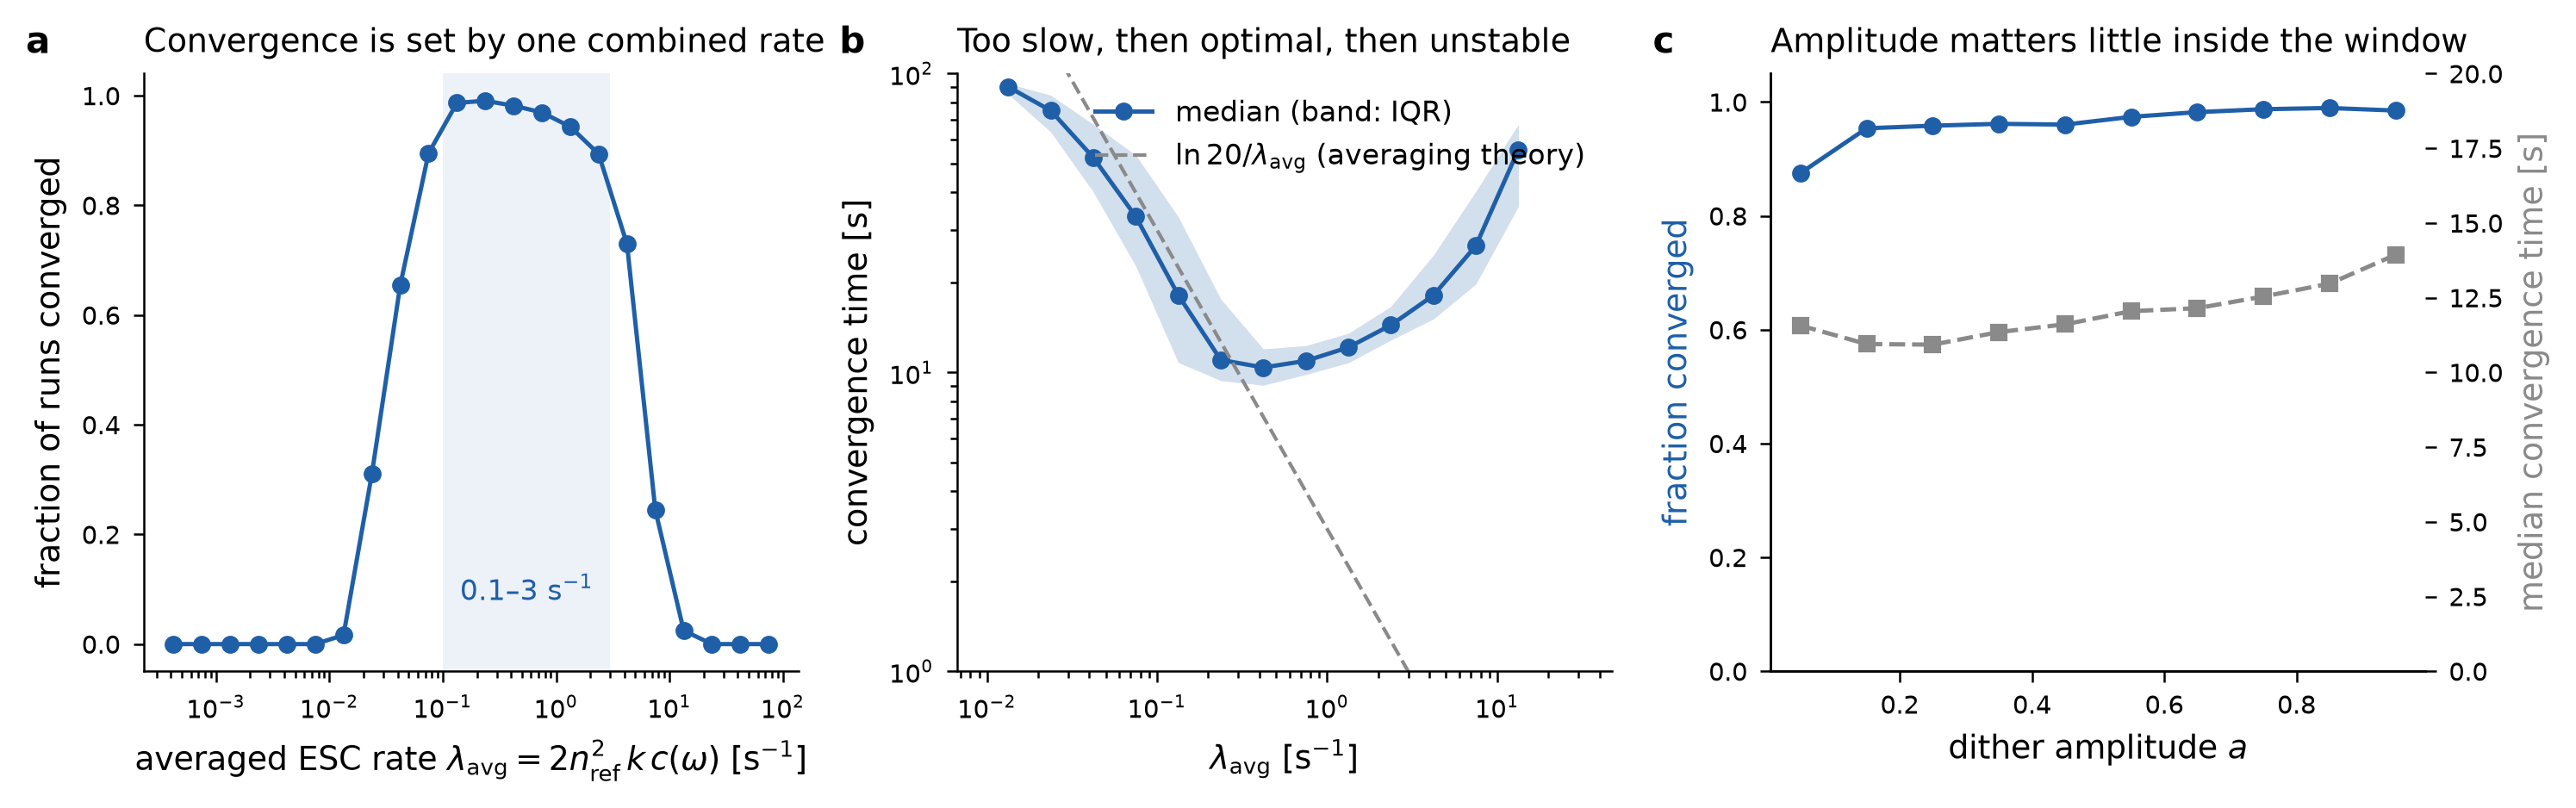
\includegraphics[width=\linewidth]{sto_effective_rate.png}
  \caption{STO 200k sweep (constant plant, $\rhat_0=0$, $n=\num{200000}$) re-expressed through the averaged rate $\lavg$ of Eq.~\eqref{eq:lavg}. (a) Fraction of runs converging within \SI{100}{s}, in bins of $0.25$ decades (each bin $\ge594$ runs). (b) Median and interquartile range of the convergence time of converged runs; dashed: $\ln20/\lavg$. At low $\lavg$ only the faster runs converge before \SI{100}{s}, which biases the median low. (c) Inside the window $0.1\le\lavg\le\SI{3}{s^{-1}}$ ($n=\num{51852}$): fraction converged (left axis) and median convergence time (right axis) versus dither amplitude. Figure generated from the repository CSV; no new simulations.}
  \label{fig:sto}
\end{figure}

\paragraph{Random loss rates.} With loss times randomised by $\pm\SI{0.1}{s}$, only \SI{25.4}{\percent} of the \num{10000} runs converge (median \SI{30.7}{s}; 178 runs below \SI{10}{s}). Even inside the $\lavg$ window, only \SI{53}{\percent} converge. Two factors contribute and cannot be separated with the stored data. (i) This sweep uses low dither frequencies ($f\le\SI{0.5}{Hz}$), where convergence is less reliable even for a constant plant. (ii) The D/T actuators are swapped in this script (Section~\ref{sec:issues}). The controller then converges to $1-\rid$ while convergence is checked against $\rid$. With $\rid$ ranging over about $0.48$--$0.54$, this mismatch can exceed the \SI{5}{\percent} band. \todo{rerun with the swap fixed and the decay rates saved per run.}
When the 178 fastest parameter sets were re-simulated (\texttt{appended\_data.csv}, column \texttt{alternative\_convergence\_time}), the median time rose from \SI{8.2}{s} to \SI{12.3}{s}. Part of their speed was therefore due to the particular decay-rate draw. \todo{confirm how the alternative times were generated.}

\subsection{Optimal-to-operate: energy and the comparison with $r=0.5$}
\label{sec:oto}

\paragraph{Random ESC parameters, random plants.} Over the 200k OTO sweep, ESC beats the fixed ratio in \SI{74.9}{\percent} of runs. This figure is not meaningful on its own: the median gain is only $1.3$ energy units ($<\SI{0.04}{\percent}$). Moreover, \SI{27.5}{\percent} of runs start inside the convergence band, because $\rhat_0=0.5$ and $\rid\approx0.5$.
The energy outcome is explained by the two quantities of Section~\ref{sec:esc} (Fig.~\ref{fig:oto}a):
\begin{itemize}
  \item The dither loss $L_\mathrm{dith}$ (Eq.~\eqref{eq:ditherloss}) sets the downside. For $L_\mathrm{dith}\le1$, ESC wins in \SIrange{91}{94}{\percent} of runs. For $L_\mathrm{dith}\in(3,10]$ it wins in \SI{45}{\percent}, and for $L_\mathrm{dith}>100$ in \SI{0.4}{\percent}, with median losses of hundreds of units.
  \item The rate $\lavg$ sets the upside. Runs with $\lavg>\SI{10}{s^{-1}}$ win in only \SI{9}{\percent} of cases (median loss 168 units), because the unstable loop throws $r$ around.
\end{itemize}
Restricting to \emph{well-tuned} runs ($0.1\le\lavg\le\SI{3}{s^{-1}}$ and $L_\mathrm{dith}<1$; \SI{16}{\percent} of the sweep) raises the win rate to \SI{93.5}{\percent} (median gain 12.2). Within this set, very small amplitudes still fail occasionally. A loss of more than 10 units occurs in \SI{29}{\percent} of runs with $a\le0.01$ and \SI{4.3}{\percent} with $a\in(0.05,0.1]$, but in none with $a>0.2$. A plausible cause is that the start-up transient of $\nD\nT$ passes the high-pass filter and is amplified by the demodulation gain $2/a$ \todo{verify on a single run}.

\paragraph{One tuned parameter set on random plants.} Based on the 3-D scatter plots, the set $k=1$, $a=0.2$, $f=\SI{6}{Hz}$ was chosen ($\lavg=\SI{1.26}{s^{-1}}$, $L_\mathrm{dith}=0.066$). On \num{100000} random plants it converged in every run (median \SI{6.8}{s}, maximum \SI{9.7}{s}). It beat $r=0.5$ in \SI{98.4}{\percent} of plants, with median gain 13.1 units. The worst case was a loss of only $0.37$ units ($\approx\SI{0.01}{\percent}$; Fig.~\ref{fig:oto}b). The gain grows with $|r_{\mathrm{ideal},0}-0.5|$ and with drift away from $0.5$, as Eq.~\eqref{eq:fixedloss} predicts. The few losses occur where $\rid$ stays near $0.5$ for the whole run.

\paragraph{Fixed plants.} For six fixed plants (Fig.~\ref{fig:oto}c), well-tuned ESC wins in \SIrange{96.0}{99.2}{\percent} of runs and recovers most of the attainable margin. For static plants with $\rid=0.475$ or $0.525$, the median gain is $6.6$ or $8.4$ units, against an upper bound of $8.5$ or $9.5$. For strongly drifting plants the gains are $111$ (bound $114$) and $165$ (bound $167$), i.e.\ \SIrange{3.5}{5.3}{\percent} of $E_{r=0.5}$.
Including untuned parameter sets, the win rates are \SIrange{70}{91}{\percent}. The notebooks note that mirror-image plants ($\rid<0.5$ versus $>0.5$) produce similar but not identical decision regions. Under the parametrisation~\eqref{eq:drift}, the static map itself is mirror-symmetric: $J(r;\rid)=J(1-r;1-\rid)$. The asymmetry must therefore come from elsewhere. Two candidates are (i) the D-rich initial state ($r=0.1$) shared by all runs, and (ii) the exponential drift, which is not mirror-symmetric: $0.55\,e^{0.2}=0.672$, whereas $1-0.45\,e^{-0.2}=0.632$. \todo{separate the two effects; for the $\lambda=0$ pair (0.475/0.525) only (i) applies.}

\begin{figure}[t]
  \centering
  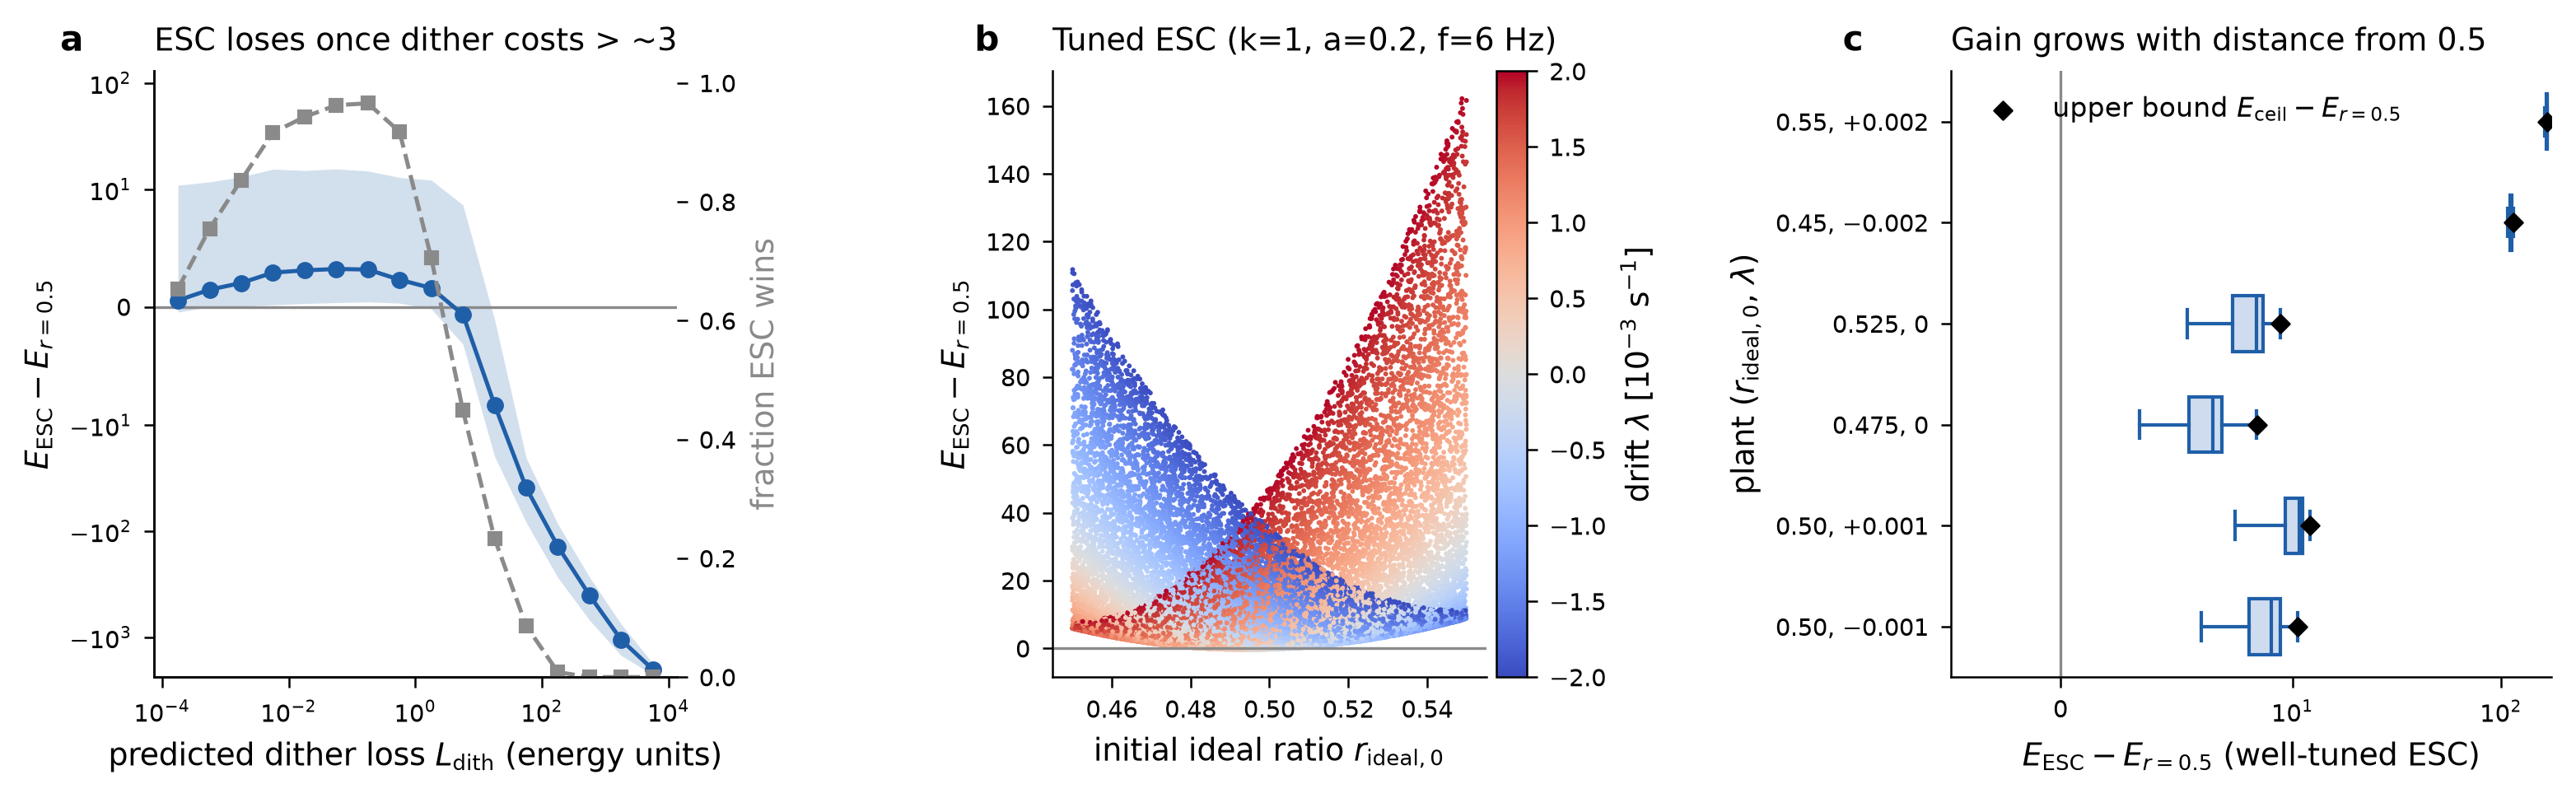
\includegraphics[width=\linewidth]{oto_energy.png}
  \caption{Energy gain of ESC over a fixed ratio $r=0.5$. (a) OTO 200k sweep ($n=\num{200000}$): median and IQR of $E_\mathrm{ESC}-E_{r=0.5}$ (symmetric-log axis) and fraction of runs in which ESC wins, in bins of the predicted dither loss $L_\mathrm{dith}$ (Eq.~\eqref{eq:ditherloss}). (b) Fixed ESC ($k=1$, $a=0.2$, $f=\SI{6}{Hz}$) on random plants; \num{20000} of \num{100000} runs shown, coloured by drift rate $\lambda$. (c) Six fixed plants, well-tuned runs only ($0.1\le\lavg\le\SI{3}{s^{-1}}$, $L_\mathrm{dith}<1$; $\approx\num{16000}$ runs each). Boxes show quartiles, whiskers 1.5\,IQR; diamonds show the upper bound $E_\mathrm{ceil}-E_{r=0.5}$. Figure generated from the repository CSVs; no new simulations.}
  \label{fig:oto}
\end{figure}

\subsection{Classifiers for convergence and for choosing ESC}
\label{sec:ml}
Fully connected networks (PyTorch: $32$-$16$ and $64$-$32$-$16$ ReLU layers; Keras for the random-decay set) were trained on 60/20/20 splits. The inputs were the ESC parameters plus engineered features ($\log_{10}k$, $\sin f$, $k\,a\sin f$). Table~\ref{tab:ml} compares the reported accuracies with the accuracy of always predicting the majority class, which is the relevant baseline for these imbalanced labels.

\begin{table}[t]
  \centering
  \small
  \caption{Classifier accuracies reported in the notebooks. Majority baseline: accuracy of always predicting the most frequent class on the same evaluation set.}
  \label{tab:ml}
  \begin{tabular}{@{}lllccc@{}}
    \toprule
    Data set & Target & Model & Train & CV / test & Majority \\
    \midrule
    STO const.\ decay 10k & converged & 32-16 & 0.969 & 0.969 & 0.710 \\
                          &           & 64-32-16 & 0.975 & 0.974 & 0.710 \\
    STO random decay 10k  & converged & Keras, 3 variants & 0.900--0.909 & 0.891--0.906 & 0.746 \\
    OTO 10k               & choose\_ESC & 32-16 & 0.931 & 0.914 & 0.753 \\
                          &             & 64-32-16 & 0.929 & 0.913 & 0.753 \\
    OTO plant $(0.5,+0.001)\to(0.5,-0.001)$ & choose\_ESC & 32-16 & 0.988 & 0.962 (test) & 0.746 \\
    OTO plant $(0.55,+0.002)\to(0.45,-0.002)$ & choose\_ESC & 32-16 & 0.995 & 0.930 (test) & 0.843 \\
    \bottomrule
  \end{tabular}
\end{table}

All classifiers beat the majority baseline, but the margin is smaller than the raw accuracy suggests. This is clearest for transfer to the mirror plant ($0.930$ versus $0.843$): recall on class 0 drops to $0.56$, so the model trained on one plant mislabels many losing parameter sets on its mirror twin.
For the random-decay set, train and CV accuracy are equal at $\approx0.90$, and adding layers did not help. This points to label noise rather than underfitting, and is consistent with the random decay rates and the D/T swap discussed above.
Given Section~\ref{sec:sto}, a physics-informed feature such as $\log\lavg$ (and $\log L_\mathrm{dith}$ for energy) is a natural input to try next \todo{test}.

%======================================================================
\section{Discussion}
\label{sec:discussion}
%======================================================================

\subsection{Should we choose ESC over $r=0.5$?}
Within this model, the answer depends on how far, and how variably, $\rid$ sits from $0.5$:
\begin{enumerate}
  \item \textbf{Static plant near $0.5$.} The prize is $(1-2\rid)^2$ of the output (Eq.~\eqref{eq:fixedloss}): \SI{0.25}{\percent} for $\rid=0.475$. A well-tuned ESC recovers most of it. A poorly tuned ESC can lose far more, either through the dither (\SI{0.94}{\percent} for the default $a=0.1$, \SI{0.1}{Hz}) or through instability. If $\rid$ were known to be within $\pm0.025$ of $0.5$, fixing $r=0.5$ would be a defensible, zero-risk choice.
  \item \textbf{Uncertain or drifting plant.} The prize grows quadratically with the offset, to \SIrange{3.5}{5.3}{\percent} for the drifting plants studied. The fixed ratio has no way to follow it. Here ESC is clearly preferable.
  \item \textbf{Risk.} The tuned set ($k=1$, $a=0.2$, $f=\SI{6}{Hz}$) lost energy in \SI{1.6}{\percent} of plants, by at most \SI{0.01}{\percent} of the output. With this tuning ESC is essentially a free option in this model.
\end{enumerate}
In short, \textbf{ESC is worth using if it is tuned inside the window} $0.1\lesssim\lavg\lesssim\SI{3}{s^{-1}}$, with a dither frequency well above the plant corner ($f\gtrsim\SI{1}{Hz}$, so that $L_\mathrm{dith}\ll1$) and $a\gtrsim0.1$. Outside this window, a fixed $r=0.5$ is often better.

\subsection{Tuning rules suggested by the data}
\begin{itemize}
  \item Choose $f$ first: high enough that the dither loss (Eq.~\eqref{eq:ditherloss}) is negligible, and well separated from the closed-loop rate.
  \item Then choose $k$ from Eq.~\eqref{eq:lavg} so that $\lavg\approx\SIrange{0.3}{1}{s^{-1}}$. This, not $k$ alone, is the quantity to report.
  \item Keep $a\gtrsim0.1$ to avoid amplifying start-up transients through $2/a$. Beyond that, $a$ has little effect on speed in this model. In a real machine $a$ will be bounded below by measurement noise and above by the acceptable perturbation of $r$.
\end{itemize}

\subsection{Limitations of the present model}
\begin{itemize}
  \item The plasma is linear and first order, with no noise, measurement delay or actuator limits besides $0\le r\le1$ and $S\ge0$. The high dither frequencies that look optimal here (\SIrange{6}{10}{Hz}) are only harmless because the model has no delay and no noise. A real neutron diagnostic and gas-valve response will limit $f$ and reintroduce the dither cost.
  \item Temperature is constant, so $P\propto\nD\nT$ exactly.
  \item The drift model (Eq.~\eqref{eq:drift}) keeps $\alpha_D+\alpha_T$ constant and can move $\rid$ beyond the sampled initial range.
  \item The fixed-ratio benchmark uses $r=0.5$ rather than the nominal model value $\rid\approx0.507$. A fairer second benchmark would be a fixed ratio at the model-based estimate.
\end{itemize}

\subsection{Issues found in the code and data}
\label{sec:issues}
\note{Collected while reading the repository; none of them changes the main conclusions, but items 1, 5 and 6 affect specific numbers.}
\begin{enumerate}
  \item \textbf{D/T swap.} \texttt{STO\_ESC\_randdecay.m} and \texttt{intuition\_Draft.m} use $u_D=rS$, $u_T=(1-r)S$, the opposite of the definition $r=\Gamma_T/(\Gamma_T+\Gamma_D)$ used everywhere else.
  \item \textbf{Amplitude lower bound.} \texttt{1e-708} underflows to $0$ in double precision, so $a$ can be arbitrarily close to zero and $2/a$ arbitrarily large.
  \item \textbf{Inconsistent initial state.} The densities are initialised for $r=0.1$ at \SI{25}{\percent} of $\nref$, while $\rhat_0=0$ (STO) or $0.5$ (OTO). This is harmless because it is common to all runs, but it should be stated.
  \item \textbf{Plot reference.} The ``$\nT$ reference'' $r\,\nref$ in the run plots is the steady state only if $\alpha_D=\alpha_T$.
  \item \textbf{Unattainable $E_\mathrm{max}$.} See Section~\ref{sec:setup}; use $E_\mathrm{ceil}$ or a fixed-$\rid(t)$ run instead.
  \item \textbf{Decision threshold.} \texttt{choose\_ESC} counts an arbitrarily small energy difference as a win, and \SI{27.5}{\percent} of OTO runs start already ``converged'' (time 0). A margin (e.g.\ $>\SI{0.1}{\percent}$) and a convergence criterion that excludes runs starting inside the band would make both labels more meaningful.
  \item \textbf{Stale notebook outputs.} The classification outputs in \texttt{STO-const\_decay-200k.ipynb} are identical to those of the 10k notebook (2000 CV samples) and were evidently not re-run on the 200k data. \texttt{OTO-ESC-200k.ipynb} has no stored outputs. Table~\ref{tab:ml} therefore uses the 10k results.
  \item \textbf{Pending run.} \texttt{OTO\_ESC\_rand\_Plant\_fix.m} is currently configured for a plant $(0.4625, +0.0015)$ whose CSV is not in the repository.
  \item \textbf{Interactive script.} In \texttt{intuition\_Draft.m} the tune-mode block is not inside an \texttt{if}, and the analyse mode resets its history at every chunk.
\end{enumerate}

%======================================================================
\section{Outlook}
\label{sec:outlook}
%======================================================================
\begin{itemize}
  \item Validate Eqs.~\eqref{eq:lavg} and~\eqref{eq:ditherloss} directly on single runs (convergence time and steady-state ripple versus $k$, $a$, $f$).
  \item Fix the D/T swap and re-run the random-decay sweep, storing the drawn $\alpha_D,\alpha_T$ per run.
  \item Decouple the filter cut-offs from $\omega$ and include $\omega_h,\omega_l$ in the sweeps.
  \item Add realistic complications in order of expected impact: measurement noise on the neutron signal, output delay (see the literature on ESC with delays in \texttt{Papers/}), time-varying and nonlinear loss rates, valve dynamics.
  \item Compare with discrete-time ESC and adaptive-step optimisers (e.g.\ RMSprop \citep{tieleman2012rmsprop}) and with safety-filtered ESC.
  \item Move towards the physical test set-up (cf.\ the TU/e theses in \texttt{Papers/}) \todo{add proper citations}.
\end{itemize}

%======================================================================
\section{Conclusion}
%======================================================================
For a first-order two-species density model with PI total-density control, sinusoidal ESC on the fuel ratio behaves as averaging theory predicts. Convergence is governed by one combined rate, $\lavg=2\nref^2kc(\omega)$, and is reliable for $0.1\lesssim\lavg\lesssim\SI{3}{s^{-1}}$. The dither amplitude matters little beyond $a\gtrsim0.1$, and the energy cost of the dither is negligible at high dither frequency.
Compared with a fixed ratio of $0.5$, a well-tuned ESC wins in \SIrange{93}{99}{\percent} of cases. The size of the win is bounded by $(1-2\rid)^2$: at most \SI{1}{\percent} for static plants in the studied range, and up to \SI{5}{\percent} for drifting plants. The case for ESC therefore rests on uncertainty and drift in $\rid$, which the next, more realistic models should quantify.

\bibliographystyle{plainnat}
\bibliography{references}

\end{document}
